\documentclass{standalone}
\usepackage{tikz}
\usetikzlibrary{patterns, positioning}
\usepackage[sfdefault]{ClearSans} %% option 'sfdefault' activates Clear Sans as the default text font
\usepackage[T1]{fontenc}

\begin{document}
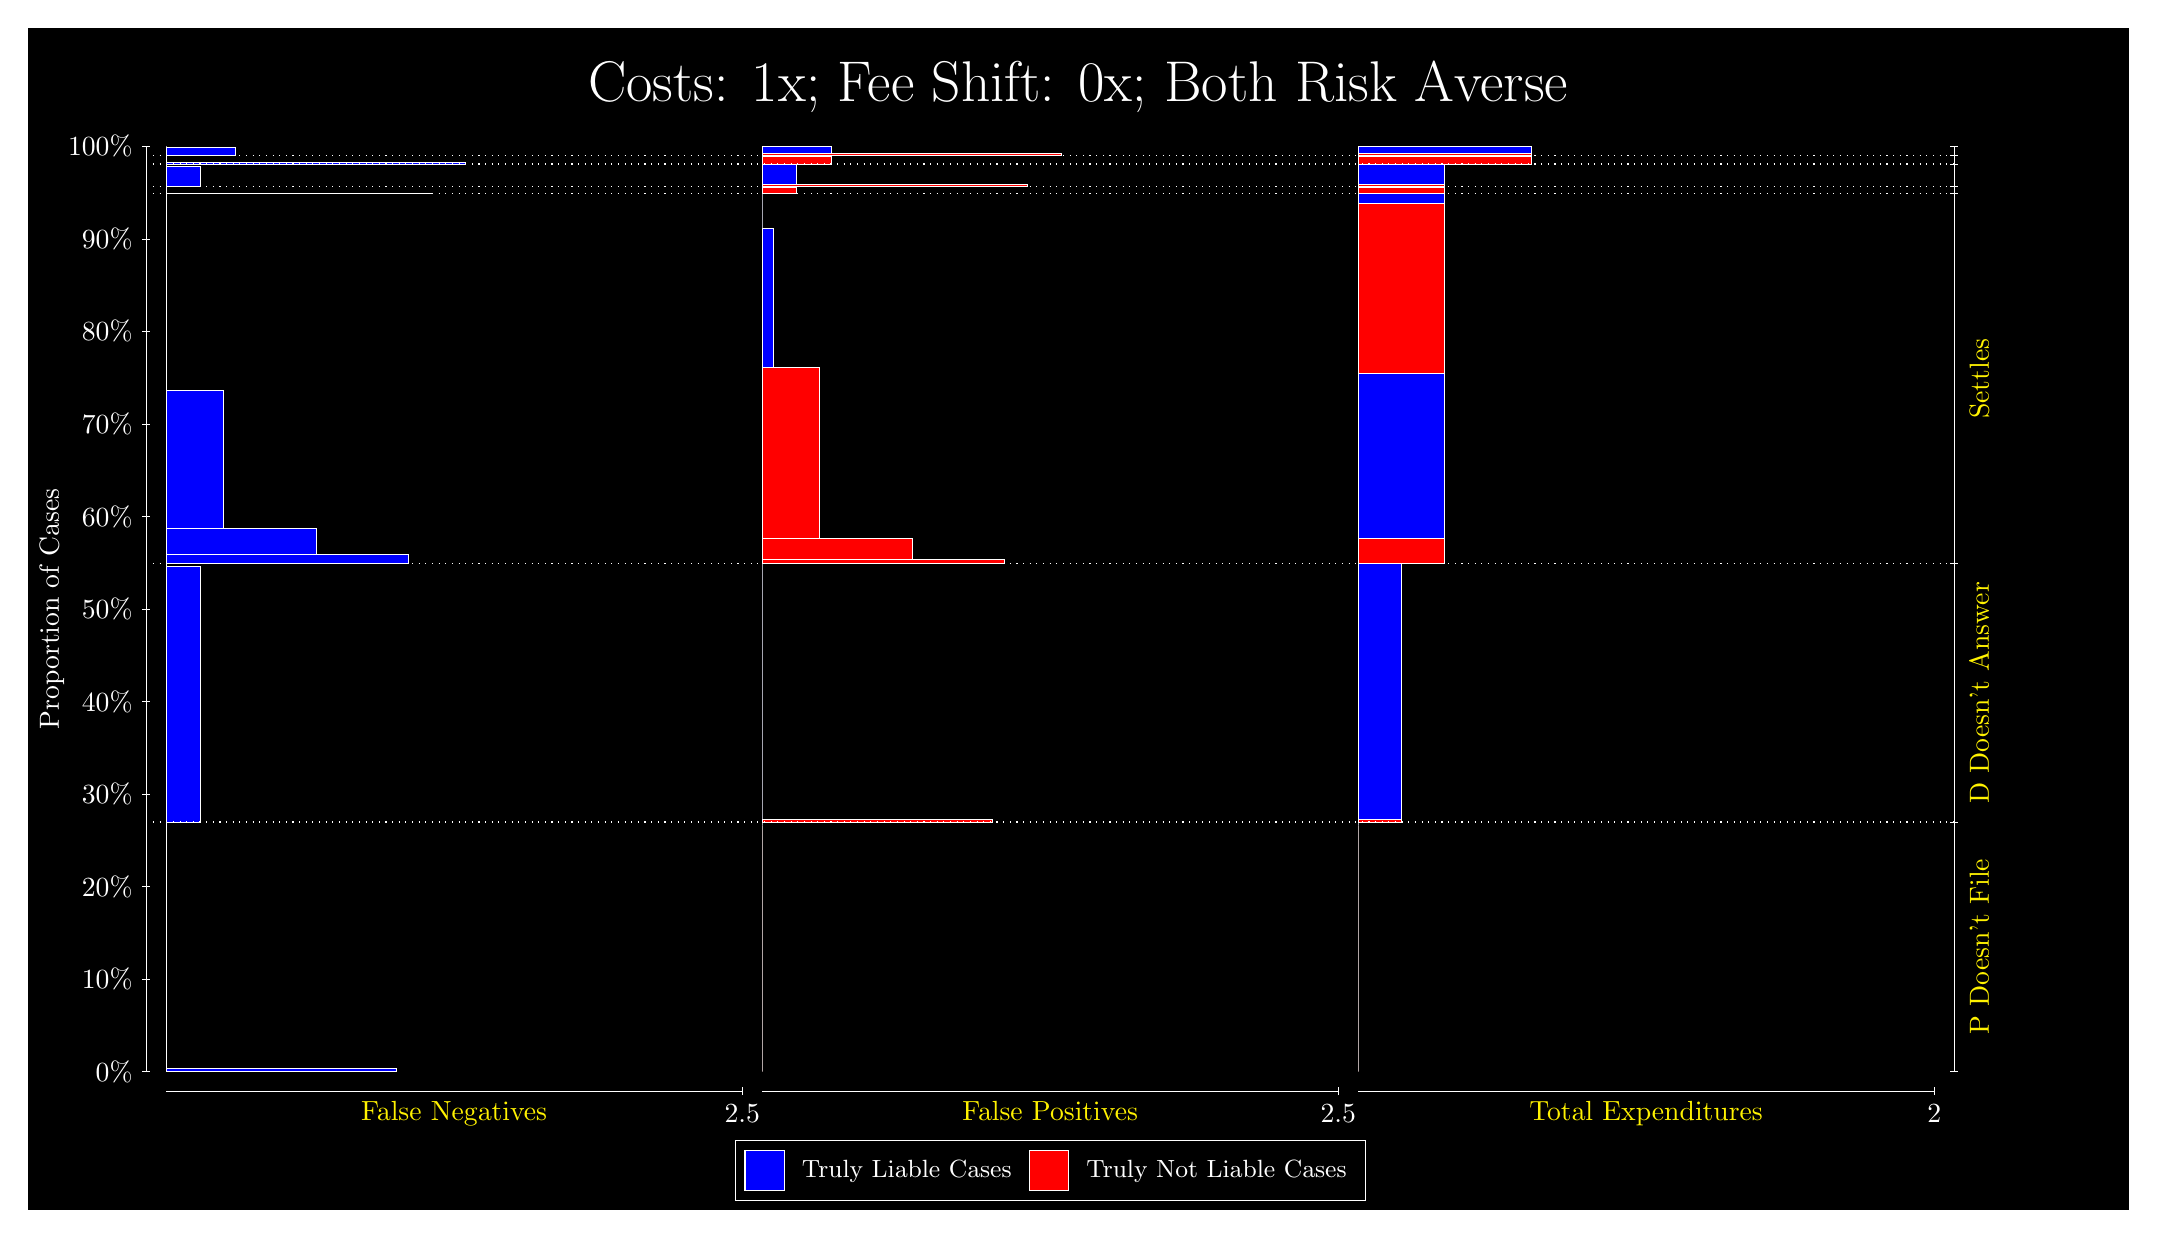
\begin{tikzpicture}
\draw[fill=black] (0,0) rectangle (26.667,15);
\draw[text=white] (0,13.5) rectangle (26.667,15) node[midway] {\huge Costs: 1x; Fee Shift: 0x; Both Risk Averse};
\draw[white, very thin] (1.5,1.75) -- (1.5,13.5);
\node[rotate=90, text=white, anchor=center] at (0.3, 7.625) {Proportion of Cases};
\draw[white, very thin] (1.45,1.75) -- (1.55,1.75);
\node[text=white, anchor=east] at (1.45, 1.75) {0\%};
\draw[white, very thin] (1.45,2.925) -- (1.55,2.925);
\node[text=white, anchor=east] at (1.45, 2.925) {10\%};
\draw[white, very thin] (1.45,4.1) -- (1.55,4.1);
\node[text=white, anchor=east] at (1.45, 4.1) {20\%};
\draw[white, very thin] (1.45,5.275) -- (1.55,5.275);
\node[text=white, anchor=east] at (1.45, 5.275) {30\%};
\draw[white, very thin] (1.45,6.45) -- (1.55,6.45);
\node[text=white, anchor=east] at (1.45, 6.45) {40\%};
\draw[white, very thin] (1.45,7.625) -- (1.55,7.625);
\node[text=white, anchor=east] at (1.45, 7.625) {50\%};
\draw[white, very thin] (1.45,8.8) -- (1.55,8.8);
\node[text=white, anchor=east] at (1.45, 8.8) {60\%};
\draw[white, very thin] (1.45,9.975) -- (1.55,9.975);
\node[text=white, anchor=east] at (1.45, 9.975) {70\%};
\draw[white, very thin] (1.45,11.15) -- (1.55,11.15);
\node[text=white, anchor=east] at (1.45, 11.15) {80\%};
\draw[white, very thin] (1.45,12.325) -- (1.55,12.325);
\node[text=white, anchor=east] at (1.45, 12.325) {90\%};
\draw[white, very thin] (1.45,13.5) -- (1.55,13.5);
\node[text=white, anchor=east] at (1.45, 13.5) {100\%};

\draw[white, very thin] (24.457,1.75) -- (24.457,13.5);
\draw[white, very thin] (24.407,1.75) -- (24.507,1.75);
\node[anchor=west] at (24.407, 1.75) {};
\draw[white, very thin] (24.407,4.9196) -- (24.507,4.9196);
\node[anchor=west] at (24.407, 4.9196) {};
\draw[white, very thin] (24.407,8.1999) -- (24.507,8.1999);
\node[anchor=west] at (24.407, 8.1999) {};
\draw[white, very thin] (24.407,12.899) -- (24.507,12.899);
\node[anchor=west] at (24.407, 12.899) {};
\draw[white, very thin] (24.407,12.992) -- (24.507,12.992);
\node[anchor=west] at (24.407, 12.992) {};
\draw[white, very thin] (24.407,13.275) -- (24.507,13.275);
\node[anchor=west] at (24.407, 13.275) {};
\draw[white, very thin] (24.407,13.388) -- (24.507,13.388);
\node[anchor=west] at (24.407, 13.388) {};
\draw[white, very thin] (24.407,13.5) -- (24.507,13.5);
\node[anchor=west] at (24.407, 13.5) {};

\draw[white, very thin, fill=blue] (1.75,1.75) rectangle (4.6775,1.794);
\draw[white, very thin, fill=red] (1.75,1.794) rectangle (1.75,4.9196);
\draw[white, very thin, fill=blue] (1.75,4.9196) rectangle (2.1891,8.1627);
\draw[white, very thin, fill=red] (1.75,8.1627) rectangle (1.75,8.1999);
\draw[white, very thin, fill=blue] (1.75,8.1999) rectangle (4.8239,8.3202);
\draw[white, very thin, fill=blue] (1.75,8.3202) rectangle (3.6529,8.6445);
\draw[white, very thin, fill=blue] (1.75,8.6445) rectangle (2.4819,10.405);
\draw[white, very thin, fill=red] (1.75,10.405) rectangle (1.75,12.899);
\draw[white, very thin, fill=blue] (1.75,12.899) rectangle (5.1167,12.909);
\draw[white, very thin, fill=red] (1.75,12.909) rectangle (1.75,12.992);
\draw[white, very thin, fill=blue] (1.75,12.992) rectangle (2.1891,13.252);
\draw[white, very thin, fill=red] (1.75,13.252) rectangle (1.75,13.275);
\draw[white, very thin, fill=blue] (1.75,13.275) rectangle (5.5558,13.293);
\draw[white, very thin, fill=red] (1.75,13.293) rectangle (1.75,13.388);
\draw[white, very thin, fill=blue] (1.75,13.388) rectangle (2.6283,13.482);
\draw[white, very thin, fill=red] (1.75,13.482) rectangle (1.75,13.5);
\draw[white, very thin, fill=red] (9.3189,1.75) rectangle (9.3189,4.8756);
\draw[white, very thin, fill=blue] (9.3189,4.8756) rectangle (9.3189,4.9196);
\draw[white, very thin, fill=red] (9.3189,4.9196) rectangle (12.246,4.9569);
\draw[white, very thin, fill=blue] (9.3189,4.9569) rectangle (9.3189,8.1999);
\draw[white, very thin, fill=red] (9.3189,8.1999) rectangle (12.393,8.2535);
\draw[white, very thin, fill=red] (9.3189,8.2535) rectangle (11.222,8.5285);
\draw[white, very thin, fill=red] (9.3189,8.5285) rectangle (10.051,10.693);
\draw[white, very thin, fill=blue] (9.3189,10.693) rectangle (9.4652,12.454);
\draw[white, very thin, fill=blue] (9.3189,12.454) rectangle (9.3189,12.899);
\draw[white, very thin, fill=red] (9.3189,12.899) rectangle (9.758,12.982);
\draw[white, very thin, fill=blue] (9.3189,12.982) rectangle (9.3189,12.992);
\draw[white, very thin, fill=red] (9.3189,12.992) rectangle (12.686,13.015);
\draw[white, very thin, fill=blue] (9.3189,13.015) rectangle (9.758,13.275);
\draw[white, very thin, fill=red] (9.3189,13.275) rectangle (10.197,13.369);
\draw[white, very thin, fill=blue] (9.3189,13.369) rectangle (9.3189,13.388);
\draw[white, very thin, fill=red] (9.3189,13.388) rectangle (13.125,13.406);
\draw[white, very thin, fill=blue] (9.3189,13.406) rectangle (10.197,13.5);
\draw[white, very thin, fill=red] (16.888,1.75) rectangle (16.888,4.8756);
\draw[white, very thin, fill=blue] (16.888,4.8756) rectangle (16.888,4.9196);
\draw[white, very thin, fill=red] (16.888,4.9196) rectangle (17.437,4.9569);
\draw[white, very thin, fill=blue] (16.888,4.9569) rectangle (17.437,8.1999);
\draw[white, very thin, fill=red] (16.888,8.1999) rectangle (17.986,8.5285);
\draw[white, very thin, fill=blue] (16.888,8.5285) rectangle (17.986,10.614);
\draw[white, very thin, fill=red] (16.888,10.614) rectangle (17.986,12.779);
\draw[white, very thin, fill=blue] (16.888,12.779) rectangle (17.986,12.899);
\draw[white, very thin, fill=red] (16.888,12.899) rectangle (17.986,12.982);
\draw[white, very thin, fill=blue] (16.888,12.982) rectangle (17.986,12.992);
\draw[white, very thin, fill=red] (16.888,12.992) rectangle (17.986,13.015);
\draw[white, very thin, fill=blue] (16.888,13.015) rectangle (17.986,13.275);
\draw[white, very thin, fill=red] (16.888,13.275) rectangle (19.083,13.369);
\draw[white, very thin, fill=blue] (16.888,13.369) rectangle (19.083,13.388);
\draw[white, very thin, fill=red] (16.888,13.388) rectangle (19.083,13.406);
\draw[white, very thin, fill=blue] (16.888,13.406) rectangle (19.083,13.5);
\draw[white, dotted] (1.5,4.9196) -- (24.457,4.9196);
\draw[white, dotted] (1.5,8.1999) -- (24.457,8.1999);
\draw[white, dotted] (1.5,12.899) -- (24.457,12.899);
\draw[white, dotted] (1.5,12.992) -- (24.457,12.992);
\draw[white, dotted] (1.5,13.275) -- (24.457,13.275);
\draw[white, dotted] (1.5,13.388) -- (24.457,13.388);
\draw[white, very thin] (1.75,1.5) -- (9.0689,1.5);
\node[text=yellow, anchor=north] at (5.4094, 1.5) {False Negatives};
\draw[white, very thin] (9.0689,1.45) -- (9.0689,1.55);
\node[text=white, anchor=north] at (9.0689, 1.45) {2.5};

\draw[white, very thin] (9.3189,1.5) -- (16.638,1.5);
\node[text=yellow, anchor=north] at (12.978, 1.5) {False Positives};
\draw[white, very thin] (16.638,1.45) -- (16.638,1.55);
\node[text=white, anchor=north] at (16.638, 1.45) {2.5};

\draw[white, very thin] (16.888,1.5) -- (24.207,1.5);
\node[text=yellow, anchor=north] at (20.547, 1.5) {Total Expenditures};
\draw[white, very thin] (24.207,1.45) -- (24.207,1.55);
\node[text=white, anchor=north] at (24.207, 1.45) {2};

\node[text=yellow, centered, rotate=90] at (24.777, 3.3348) {P Doesn't File};
\node[text=yellow, centered, rotate=90] at (24.777, 6.5598) {D Doesn't Answer};
\node[text=yellow, centered, rotate=90] at (24.777, 10.549) {Settles};





\draw (12.978300999999998,1.5) node[draw=none] (baseCoordinate) {};
\begin{scope}[align=center]
        \matrix[scale=0.5, draw=white, below=0.5cm of baseCoordinate, nodes={draw}, column sep=0.1cm]{
            \node[rectangle, draw, minimum width=0.5cm, minimum height=0.5cm, fill=blue] {}; &
            \node[draw=none, font=\small, text=white] (B) {Truly Liable Cases}; &
            \node[rectangle, draw, minimum width=0.5cm, minimum height=0.5cm, fill=red] {}; &
            \node[draw=none, font=\small, text=white] (B) {Truly Not Liable Cases}; \\
            };
\end{scope}

\end{tikzpicture}
\end{document}